\section{Overview of the Silicon Tracking System}
\subsection{Role of the tracker}
\subsection{Silicon Sensors}
\label{sensors}
One of the important parameters of the silicon sensor is leakage current, which is strongly correlated with the temperature as per equation \ref{Sil:temp} \cite{Hartmann:2017gzy}.

\begin{equation}
\label{Sil:temp}
    I_{R}(T) \propto T^{2}e^{\frac{-E}{2kT}}
\end{equation}
 By assuming that one of the  temperature sensors at a similar height as the silicon sensors mimics their temperature. This assumption clearly doesn't consider several effects like silicon sensors' self-heating. Nevertheless, it allows us to scale down leakage current to $20\,^{\circ}$C using the equation \ref{Sil:scal}.
 
\begin{equation}
\label{Sil:scal}
    \frac{I_{R}(T_{2})}{I_{R}(T_{1})} = (\frac{T_{2}}{T_{1}})^{2}e^{\frac{-E}{2kT}\frac{T_{1}-T_{2}}{T_{1}T_{2}}}
\end{equation}

\begin{figure}[!h]
\centering
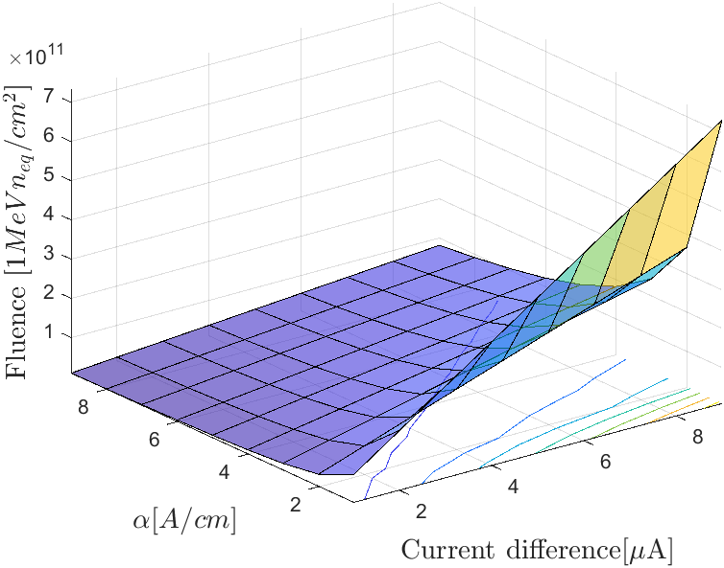
\includegraphics[width=0.65\columnwidth]{Chapter2/images/Leakage_current.png}
\caption{The first proposition of the CBM readout chain based on separate DPB and FLIB boards \cite{CRI}}
\label{fig_leakage}
\end{figure}

\begin{figure}[!h]
\centering
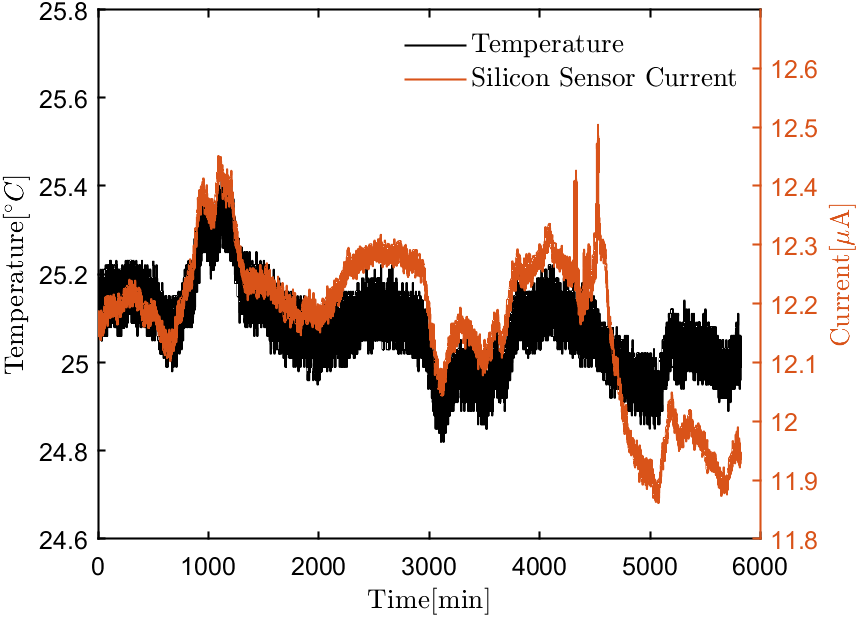
\includegraphics[width=0.65\columnwidth]{Chapter2/images/currenttempnobeam.png}
\caption{The first proposition of the CBM readout chain based on separate DPB and FLIB boards \cite{CRI}}
\label{fig_leakage1}
\end{figure}



\subsection{Module}
\subsection{STS-XYTER}
\subsection{Front End Boards}
\label{module}
\subsection{Readout chains}
\label{DAQ}
There are three main readout chains that have been exercised for different detector development activities.  
The readout chain used in the module or FEBs test is built from two components: 
\begin{enumerate}
    \item the Common Readout Board (\gls{CROB}) for data concentration and transport with electrical to optical interface (see figure \ref{fig_crob}.
    \item Data Processing Board (DPB) based on the AFCK board (see Fig.~\ref{afck_pic})
\end{enumerate}

\begin{figure}[!h]
\centering
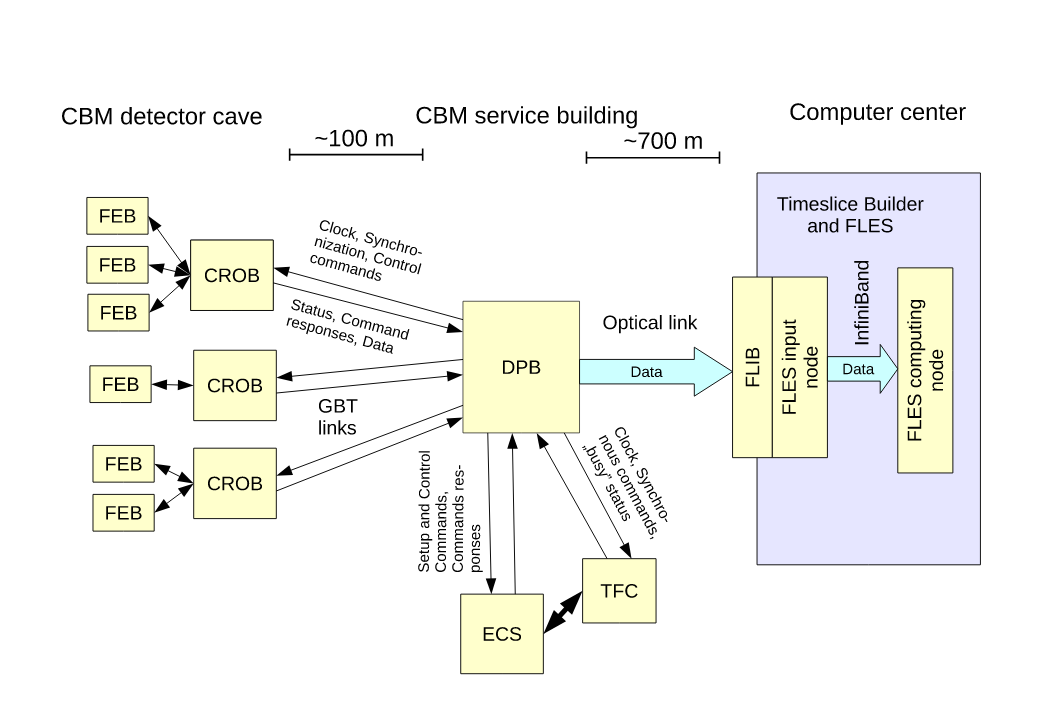
\includegraphics[width=0.65\columnwidth]{Chapter2/images/DPB.png}
\caption{The first proposition of the CBM readout chain based on separate DPB and FLIB boards \cite{CRI}}
\label{fig_dpb_scheme}
\end{figure}

\begin{figure}[!h]
\centering
\includegraphics[width=0.65\columnwidth]{Chapter2/images/feb_8_v2.pdf}
\caption{FEB}
\label{fig_febA_photo}
\end{figure}
\subsection{CRI based readout chain}
\begin{figure}[!h]
\centering
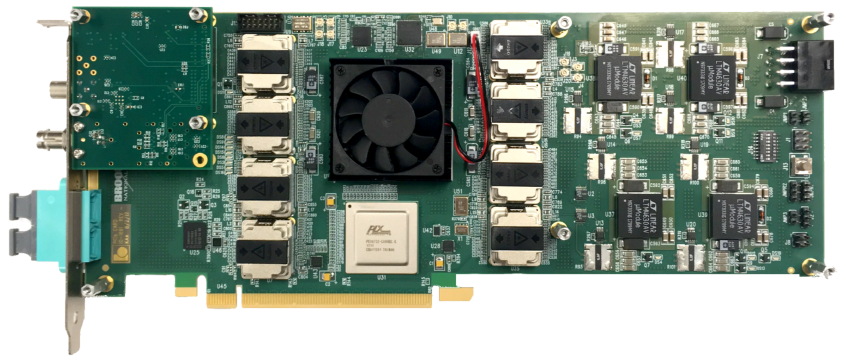
\includegraphics[width=0.65\columnwidth]{Chapter2/images/cri_board_atlas.pdf}
\caption{CRI board}
\label{fig_cri_board}
\end{figure}
\subsection{DPB based readout chain}

\subsection{Tester readout chain}
\label{tester}
Another alternative to the two readout chains introduced in the last two sections is so-called GBTxEMU-based tester. It is based on a commercial Artix-7 board (TE-0712, Trenz Electronics Gmbh), and allows emulating GBTX ASIC or the whole CROB. Moreover, it could also be used in an autonomous mode with the addition of VITA  57.1 FMC adapter

\subsection{Cooling}
\label{cooling}
\subsection{Powering scheme}
\label{powering}
\subsection{Detector enclosure}
